\chapter{Detalles de Implementación y Experimentos}\label{chapter:implementation}

%region Nomenclatura 
En este capítulo se mostrará la forma y los pasos para generar el problema deseado en el contexto de un generador de puntos estacionarios para problemas binivel. Este capítulo aborda el diseño y la implementación del generador, explicando detalladamente las metodologías empleadas, los criterios necesarios para asegurar la validez de los puntos obtenidos y los algoritmos utilizados en cada etapa del proceso.

\section{Notaciones:}
 El problema binivel optimista, definido en (\ref{eq:ProblemaGeneral}), consiste en
\begin{equation}
\begin{aligned}
& \min_{x} \; F(x, y) \\
& \text{sujeto a } \\
& g_i(x, y)\leq 0,\;i=1,\ldots,q, \\
& y \in \argmin_{y} \left\{ f(x, y) \mid v_j(x, y)\leq 0,\;j=1,\ldots,q ,\right\}
\end{aligned}
\end{equation}
Luego el modelo se puede definir usando solo las funciones 
\begin{itemize}
    \item$F(x,y)$: Función del líder.                                                                                                          \\
       \item $ g_i(x,y) $:               Restricciones de desigualdad del líder,  $ i=1,\ldots, q$.       \\
        \item $ f(x,y) $:            Función del seguidor.                                                               \\
       \item $ v_j(x,y) $:                Restricciones de desigualdad del seguidor, $j=1\ldots s$.   \\
    \end{itemize}
A este modelo se le aplicará el enfoque KKT, obteniéndose
 \begin{equation}
            \begin{array}{l}
                \underset{\substack{x, y, \lambda_j}}{\min} \quad F(x, y)\\
                s.a \left\{ 
                \begin{array}{l}
                    g_i(x, y) \leq 0, i=1\ldots q,\\
                    \nabla_{y} f(x, y) + \sum_{j=1}^{s} \nabla_{y} v_j(x, y) \lambda_j = 0, \\
                    v_j(x, y) \leq 0, j=1\ldots s,\\
                    v_j(x, y)\lambda_j = 0, j=1\ldots s, \\
                    \lambda_j \geq 0, j=1\ldots s.\\
                \end{array}\right.
            \end{array}
        \end{equation} introducido en \ref{eq:KKT_Optimista}.

La condición de estacionariedad está dada por ser la solución del sistema 

$$\begin{matrix}
 \nabla_z F(z_{est}) + \sum_{i=1}^q \mu_i\nabla_z g_i(z_{est}) +\sum_{i=1}^{s} \beta_j\nabla v_j(z_{est}) +\\+\sum_{k=1}^{q_0} \alpha_k\nabla_z[  \nabla_{y} f((z_{est}) +\sum_{j=1}^{s} \nabla_{y} v_j((z_{est}) \lambda_j]&=&0\\
 \alpha  \nabla_{y} v_j(x, y)-\gamma_j&=&0\end{matrix}$$

donde, denotando  \begin{equation}\label{activeg} J_0^g=\{i: g_i(x,y)=0\}\end{equation}    como los índices activos del líder,         $$J_0^v=\{j: v_j(x,y)=0\},$$  los del seguidor y  $$J_0^\lambda=\{j:  \lambda_j=0\},$$ como  los elementos de $\lambda$ que son 0,
  $$\begin{matrix}
        & \beta_j= 0,\; j\in \{1,\ldots, s\}\setminus J_0^v,\\
        &  \gamma_j= 0,\; j\in \{1,\ldots, s\}\setminus J_0^\lambda,  \\
        & g_i(z_{est}) \leq 0, \quad \mu_i \geq 0, \quad \mu_i g_i(z_{est}) = 0, i=1,\ldots, q.
    \end{matrix}$$ 

De esta forma  
\begin{itemize}\item$ \alpha\in \mathbb{R}^m  $: multiplicador asociado a la condición de KKT del problema de nivel inferior.                                                                                                     
       \item  $\mu_i \in \mathbb{R}^q$:  multiplicador asociado a las restricciones  $g_i(x,y)$ del líder.  \item        $ \beta_j\in \mathbb{R}^s  $:              multiplicador asociado  a las restricciones   $v_{j}$ del líder.          
   \item        $\gamma_j\in \mathbb{R}^s$:            multiplicador asociado a las  restricciones  $\lambda_j \geq 0$.\end{itemize}



Condiciones extra respecto al signo de $\beta$ y $\gamma$ se tendrán en cuenta en dependencia de si el usuario escoge que sea  C,M, fuerte estacionario o cumpla  la condición $\alpha=0$.  Es por esto que el conjunto $\{1,\ldots, s\}$  se particiona en 
 \begin{equation} 
 J_1^v=\{j | v_j(x,y)=0 \land \lambda_j>0 \} %al conjunto restricciones de desigualdad que sean índices activos
 \label{J_0_lambda_pos_level_inferior}
 \end{equation} 
 \begin{equation}
    J_2^v=\{j | v_j(x,y)=0 \land \lambda_j=0 \}
    \label{J_0_lambda_0_level_inferior}
\end{equation}
                  
 \begin{equation}
    J_3^v=\{j | v_j(x,y)< 0 \land \lambda_j=0 \}
    \label{J_neg_lambda_0_level_inferior}
\end{equation}
            
    
Cada índice activo tiene multiplicadores $\beta_j$ y en dependencia del caso $\gamma_j$ asociados. De esta forma 
$\beta_j= 0,\; j\in  J_3^v,\; \gamma_j= 0,\; j\in J_1^v.$  Las condiciones de signo de la clase de punto estacionario correspondiente se analizan para $\beta_j, \gamma_j= 0,\; j\in J_2^v.$
       

Usando estas notaciones, en la próxima sección se muestra como se genera le problema.


   %     $ v_{j}^{\star} $     Restricción de desigualdad del seguidor activa después de modificarse el problema   $j=1\ldots s$.          \\

%endregion
\section{Generación del problema sobre Julia}
A continuación se mostrarán los pasos a seguir para generar el problema deseado.
\subsection{Datos de entrada}

Lo primero  que hace el usuario es escoger si $\alpha=0$ o no. En el segundo caso se le solicita que  introduzca el valor de dicho multiplicador. Luego se
declaran las  variables diferenciando las del líder $x$ y las del seguidor $y$. Se chequea que la dimensión de   $\alpha$  y de $y$ coincidan. 

Con las variables se introduce la función objetivo del líder $F(x,y)$ y las restricciones $ g_1(x,y),\ldots, g_q(x,y)$. En cada caso el usuario define si desea que sea activa o no y para las activas  le introduce el correspondiente multiplicador $\mu_j$. De esta forma se construye el conjunto $J_0^G=\{i | g_i(x,y)=0\}$ y se logra que  $g_i(x,y)\mu_i=0$ para todo $i=1,\ldots,q$. Se le advierte al usuario que $\mu_j$ debe ser no negativo, dándole la posibilidad de cambiarlo de haber cometido un error.

De manera análoga se procede con la función objetivo del seguidor $f(x,y)$,  sus restricciones  $ v_1(x,y),\ldots, v_s(x,y)$ y sus multiplicadores $\lambda$  no negativos. Sabiendo que al menos uno de ellos $v_j(x,y)\lambda_j=0$, se construye la partición $(J_1^v,J_2^v,J_3^v)$  del conjunto $\{1,\ldots,s\}$  descrita en (\ref{J_0_lambda_pos_level_inferior}),  (\ref{J_0_lambda_0_level_inferior}),  (\ref{J_neg_lambda_0_level_inferior}).

Finalmente se introducen el resto de los multiplicadores,  a saber $\beta$ y $\gamma$,  de forma que cumplan la condición de la clase de estacionariedad correspondiente. Se consideran dos casos diferentes
\begin{itemize}
\item {\textbf{ $\alpha=0$}}: Se hace automáticamente $\gamma =0$   y el  usuario introduce el multiplicador $\beta_j, j=1,\ldots,s $ de forma tal que: 

\item[]\begin{center} {\textbf{ C-estacionario:}} \end{center}\begin{itemize}\item si $j\in J_1^v\cup J_2^v$: $\beta_j$ libre.\item si $j\in J_3^v$: $\beta_j=0$.\end{itemize}
\item[]\begin{center} {\textbf{ M-estacionario:}} \end{center}\begin{itemize}\item si $j\in J_1^v\cup J_2^v$: $\beta_j$ libre.\item si $j\in J_3^v$: $\beta_j=0$.\end{itemize}
\item[]\begin{center} {\textbf{ fuertemente-estacionario:}} \end{center}\begin{itemize}\item si $j\in J_1^v$: $\beta_j$ libre.\item si $j\in J_2^v$: $\beta_j\geq 0$.\item si $j\in J_3^v$: $\beta_j=0$.
\end{itemize}
\item  {\textbf{$\alpha\neq 0$:}} si cada $j=1,\ldots,q$ se introduce el par de multiplicadores $\beta_j, \gamma_j, j=1,\ldots,s$ de forma tal que: 
\item[]\begin{center} {\textbf{ C-estacionario:}} \end{center}\begin{itemize}\item si $j\in J_1^v$: $\beta_j$ libre, $\gamma_j=0$.\item si $j\in J_2^v$: $\beta_j\gamma_j\geq 0$.\item si $j\in J_3^v$: $\beta_j=0,\gamma_j$ libre.\end{itemize}
\item[]\begin{center} {\textbf{ M-estacionario:}} \end{center}\begin{itemize}\item si $j\in J_1^v$: $\beta_j$ libre, $\gamma_j=0$.\item si $j\in J_2^v$: $\beta_j,\gamma_j> 0$ o $\beta_j\gamma_j=0$.\item si $j\in J_3^v$: $\beta_j=0,\gamma_j$ libre.\end{itemize}
\item[]\begin{center} {\textbf{fuertemente-estacionario:}} \end{center}\begin{itemize}\item si $j\in J_1^v$: $\beta_j$ libre, $\gamma_j=0$.\item si $j\in J_2^v$: $\beta_j,\gamma_j\geq 0$.\item si $j\in J_3^v$: $\beta_j=0,\gamma_j$ libre.
\end{itemize}
\end{itemize}



% COndiciones \Beta_i \Gamma_i para puntos estacionarios

\subsection{Modificación del Problema Original}
Después de tener los datos de entrada necesarios se procede a la modificación
del problema de entrada para que este sea estacionario del tipo requerido, $z_{est}$.

%
% Decir que en caso de que \alpha != de nulo entonces se calcula b_j
Primero en caso de que $\alpha \neq 0$ en los $v_j(x,y) \in J_0^v$ se procede a calcular el $\vec{b_j}$ de la siguiente forma:

%Como calcular b_j
\begin{itemize}
    \item \textbf{ $v_j(x,y) \in J_!^v$ \ref{J_0_lambda_pos_level_inferior}}:
        \begin{equation}
            \vec{b_j}=  \frac{{\alpha} \cdot (-\nabla_{y}{v_j(z_{est})}^T \cdot \alpha)}{\|\mathbf{\alpha} \|_2^2}
        \end{equation}
    \item \textbf{$v_j(x,y) \in J_2^v \lor J_3^v$ (\ref{J_0_lambda_0_level_inferior}), (\ref{J_neg_lambda_0_level_inferior})}\\
    \begin{equation}
        \vec{b_j}=  \frac{{\alpha} \cdot ((-\nabla_{y}{v_j(z_{est})}^T \cdot \alpha)+\gamma_j)}{\|\mathbf{\alpha} \|_2^2}
    \end{equation}
\end{itemize}

Si $\alpha=0$, como $\gamma=0$, se toma  $\vec{b_j}=0$
            
Después de realizado el cálculo del $b_j$, se procede a modificar la función por una constante para lograr que sean activas en $z_{est}$ aquellas que fueron escogidas por el usuario y que todas sean no positivas. Para ello se evalua $$\hat{v_j}=v_{j}(z_{est})+ ({\vec{b_j}}^T)\cdot (y_1,y_2,\dots,y_m).$$ Se consideran los siguientes casos
\begin{itemize}
    \item Si $\hat{v_j}\neq 0$ y $j\in J_1^v\cup J_2^v$, entonces $c_j^v=-\hat{v_j}$.
\item Si $\hat{v_j}\geq 0$ y $j\in J_3^v$,  entonces  $c_j^v$ se obtiene generando un número aleatorio entre $(-\hat{v_j}-.01, -10)$.
\item En otro caso $c_j^v=0$.\end{itemize}

De ahí que las restricciones del nivel inferior tengan la forma 
\begin{equation}
	v_{j}^{\star}(x,y)=v_{j}(x,y)+ ({\vec{b_j}}^T)\cdot (y_1,y_2,\dots,y_m)+c_j^v
\end{equation}
%
Con estas condiciones se logra que 
$$\begin{array}{rcll} \alpha \nabla_y v_{j}^{\star}(z_{est})&=&0,& j\in J_1^v,\\ \alpha \nabla_y v_{j}^{\star}(z_{est})-\gamma_j&=&0,& j\in J_2^v\cup J_3^v,\\
  v_{j}^{\star}(z_{est})&=&0,& j\in J_1^v\cup J_2^v, \\  v_{j}^{\star}(z_{est})&<&0,& j\in J_3^v.\end{array}$$

% Explicar que se hace el punto factible en las restricciones
De forma análoga se agregan constantes  $c_i^g$  a las restricciones del líder,  teniéndose que para $$g_{i}^{\star}(x,y)=g_{i}(x,y)+c_i^g,$$ se cumple

$$\begin{array}{rcll} 
  g_{i}^{\star}(z_{est})&=&0,& j\in J_0^g,\\  g_{i}^{\star}(z_{est})&<&0,& j\in \{1, \ldots, q\}\setminus J_0^g.\end{array}$$

Solo falta lograr el cumplimiento de las condiciones de KKT del problema del seguidor. Para ello se considera el sistema 

\begin{equation}
    \begin{aligned}
        &\nabla_{y}f(z_{est})+\sum_{j \in J_2^v}(\lambda_j\nabla_{y}v_{j}^{\star}(z_{est}))+\vec{bf}=\vec{0}.\\
        &\text{KKT del problema del nivel inferior}
    \end{aligned}
    \label{KKT_nivel_inferior}
\end{equation}

De esta manera la función objetivo del seguidor es
$$f^{\star}(x,y)=f(x,y)+\vec{bf}y$$


%Explicar que como se había hallado ya el KKT del level inf ahora se puede realizar completo
Finalmente se toman  las derivadas del sistema de KKT con respecto a $(x,y)$. Para ello  se considera el sistema
% MPEC all KKT 
 
    $$
       \nabla_{xy}F(z_{est})+\sum_{j\in J_o^g|}(\mu_i\nabla_{xy}g(z_{est}))+[\nabla_{x,y}\nabla_{y}f(z_{est})+\sum_{j \in J_1^vg}\lambda_j\nabla_{xy}\nabla_{y}v_{j}^{\star}(z_{est})]\alpha+$$ $$\sum_{j \in J_1^v \cup J_2^v|}(\beta_j\nabla_{xy}v_{j}^{\star}(z_{est})+\vec{BF}=\vec{0},
   $$
y se obtiene

$$F^{\star}(x,y)=F(x,y)+\vec{BF}(x,y)^T.$$
De esta forma el problema de dos niveles 
\begin{equation}
\begin{aligned}
& \min_{x} \; F^{\star}(x, y) \\
& \text{sujeto a } \\
& g_i^{\star}(x, y)\leq 0,\;i=1,\ldots,q, \\
& y \in \argmin_{y} \left\{ f^{\star}(x, y) \mid v_j^{\star}(x, y)\leq 0,\;j=1,\ldots,q ,\right\}
\end{aligned}
\end{equation}
cumple que el punto $(z_{est},\lambda_{est})$ es un punto estacionario del modelo MPEC correspondiente.

La salida del generador son las funciones $F^{\star}(x,y), f^{\star}(x,y),$, $g_1^{\star}(x,y),\ldots,g_q^{\star}(x,y)$, $v_1^{\star}(x,y),\ldots,v_s^{\star}(x,y)$.
% Explicación algorítmica y manual de usuario

\section{Implementación Algorítmica y Guía de Usuario}
%region Introducción de la sección
En la implementación computacional del generador propuesto en la sección anteriores
se utilizó el lenguaje de programación \textbf{Julia}, ver \cite{Juliadocs}, dado a su versatilidad
en expresiones y funciones matemáticas implementadas en su paquete base y sus bibliotecas externas como 
\textbf{BilevelJuMP}, ver \cite{BilevelJump}, que permite resolver problemas binivel SLSF lineales y cuadráticos
sin tener que transformar el problema original y \textbf{JuMP} \cite{JuMPPaper} el cual, es una interfaz robusta para la optimización general,
todo ello con unas excelentes prestaciones de cómputo. Por ello se brinda una guía de usuario para el uso del generador disponible en 
\href{https://fvsb.github.io/Tesis/}{https://fvsb.github.io/Tesis/}.  

%\subsection{Guía de Usuario}
% Después compilar a ProblemGenerator
La implementación algorítmica se ha llevado a cabo mediante la creación de una biblioteca de Julia
llamada \textbf{ProblemGenerator}, con una sintaxis \textit{JuMP-like} intuitiva.
Primero debe tenerse un problema de optimización Binivel SLSF planteado como el \ref{eq:DefBinivelOptimista}, el punto que se desea que sea estacionario ($z_{est}$), los índices activos descritos anteriormente 
según el caso así como sus multiplicadores correspondientes, que cumplirán las propiedades del tipo de estacionariedad requerida y la opción de tener  $\vec{\alpha}$ igual a o distinto de cero.
%endregion

%\subsection{Ejemplo a utilizar}
Para una mayor facilidad de compresión del uso de la biblioteca se utiliza este problema ejemplo:
\begin{equation}
    \begin{aligned}
        & \underset{x_1, x_2}{\text{mín}} 
        && x_1^2 y_1^2 y_2 + x_2 \\
        & \text{s.t.} 
        && x_1 + y_2 - y_1 \leq 9, \\
        & 
        && \underset{y_1, y_2}{\text{mín}} 
        \quad x_2^2 y_1^2 y_2 + x_1 \\
        & 
        && \text{s.t.} 
        \quad x_1^2 y_1^2 + x_2 \leq 0.
    \end{aligned}
    \label{ProblemaEjemplo}
\end{equation}
%Dependencias para la biblioteca
%\subsection{Dependencias}
Se debe tener instalado en el entorno de desarrollo de Julia los siguientes módulos:
%Se debe tener en cuenta que este paquete instalará las siguientes dependencias
\begin{itemize}
    \item Symbolics 
    \item LinearAlgebra
\end{itemize}

% Importar la Biblioteca
%\subsection{Importación de la biblioteca}
Para la utilización de la biblioteca se procede a su importación de la siguiente forma:
\begin{lstlisting}[caption=Importar el Módulo]
    using ProblemGenerator
\end{lstlisting}

% Crear modelo base
%\subsection{Crear el modelo base}
Para comenzar debe llamarse a la función \textbf{GeneratorModel} para crear el modelo base
inicial.

\subsubsection{Para $\vec{\alpha}=\vec{0}$ }

%Crear para alpha nulo
Para crear un modelo donde $\vec{\alpha}=\vec{0}$:
   
        \begin{lstlisting}[caption={Crear el modelo para $\vec{\alpha}=\vec{0}$}]
            # Crear el modelo base del generador alpha=0
            model=GeneratorModel()
        \end{lstlisting}
        
    
  
%Crear para alpha no nulo
%
\subsubsection{Para $\vec{\alpha} \neq \vec{0}$ }

Para crear un modelo donde $\vec{\alpha}\neq \vec{0}$,
se tiene que pasar como parámetro el valor del $\alpha$,
el cual será un vector de \textit{Number}:

\begin{lstlisting}[caption={Crear el modelo para $\vec{\alpha } \neq \vec{0}$}]
    # Crear el modelo base del generador alpha!=0
    alpha_vec=Vector::{Number}
    model=GeneratorModel(alpha_vec)
\end{lstlisting}
%



% Explicar las funciones Upper y Lower
%\subsection{Función para diferenciar los niveles}
En caso que se requiera como entrada un \textbf{Problem}, se debe declarar
de que nivel se trata de evaluar el \textbf{model} en las funciones \textbf{Upper} para el nivel 
superior y \textbf{Lower} para el inferior.

\subsubsection{Para referirse al nivel superior}
\begin{lstlisting}[caption={Referirse al nivel superior}]
    # Referirse nivel superior
    Upper(model)
\end{lstlisting}
\subsubsection{Para referirse al nivel inferior}
\begin{lstlisting}[caption={Referirse al nivel inferior}]
    # Referirse nivel inferior
    Lower(model)
\end{lstlisting}


%\subsection{Declarar Variables}
Las variables deben de 
declararse bajo la siguiente macro \textbf{@myvariables}, la cual 
recibe una función \textbf{Upper} o \textbf{Lower} que recibe el modelo
para las variables del nivel superior y las del nivel inferior respectivamente.

\subsubsection{Introduccion de  las variables del nivel superior }
%Ejemplo de introducir al level superior

\begin{lstlisting}[caption={Introducir las variables del nivel superior}]
    # Se declara en el nivel superior las variables x_1, x_2
    @myvariables Upper(model) x_1, x_2
\end{lstlisting}

\subsubsection{Introducción de las variables del nivel inferior}
%Ejemplo para introducir las variables del nivel inferior

\begin{lstlisting}[caption={Introducir las variables del nivel inferior}]
   # Se declara en el nivel inferior las variables y_1, y_2
   @myvariables Lower(model) y_1,y_2
\end{lstlisting}


%Declarar las funciones objetivo
\subsection{Declarar Funciones Objetivo}

Para declarar las funciones objetivos debe asumirse que en ambos casos es un 
problema de minimización. Se utilizará la función \textbf{SetObjectiveFunction}
que recibe un \textbf{Problem} y una expresión de \textbf{Num}.

% Declaración de Función Objetivo de nivel Superior
\subsubsection{ Declaración de una función objetivo del nivel superior}
Con: $$\min (x_1^2*y_1^2*y_2) + x_2$$
\begin{lstlisting}[caption={ Declarar una función objetivo del nivel superior}]
    # Declarar la funcion objetivo del nivel superior
    # Min de ((x_1^2)*(y_1^2)*(y_2))+x_2
    SetObjectiveFunction(Upper(model),((x_1^2)*(y_1^2)*(y_2))+x_2)
\end{lstlisting}

\subsubsection{Declaración de una función objetivo del nivel inferior}
%Declaración de Función objetivo Nivel inferior

Con: $$\min (x_2^2*y_1^2*y_2)+x_1$$
\begin{lstlisting}[caption={Declarar una función objetivo del nivel inferior.}]
    # Declarar la funcion objetivo del nivel inferior
    # Min de ((x_2^2)*(y_1^2)*(y_2))+x_1
    SetObjectiveFunction(Lower(model),((x_2^2)*(y_1^2)*(y_2))+x_1)
\end{lstlisting}

% Definición de tipo de índices activos.
\subsection{Definición del conjunto de Índices activos}

Antes de ilustrar como introducir las restricciones se va a explicar 
que los tipos de índices activos.

\begin{itemize}
    \item \textbf{Ambos Niveles}:
        \begin{itemize}
            \item \textbf{Normal} si no es un índice activo.
        \end{itemize}
    \item \textbf{Nivel Superior}:
     \begin{itemize}
        \item \textbf{J\_0\_g} Si es un índice como en (\ref{activeg}).
     \end{itemize}
    \item \textbf{Nivel Inferior}:
    \begin{itemize}
        \item \textbf{J\_0\_LP\_v} Si es un índice como en \ref{J_0_lambda_pos_level_inferior}.
        \item  \textbf{J\_0\_L0\_v} Si es un índice como en \ref{J_0_lambda_0_level_inferior}.
        \item  \textbf{J\_Ne\_L0\_v} Si es un índice como en \ref{J_neg_lambda_0_level_inferior}.
    \end{itemize}
\end{itemize}


%Ejemplo de como se debe de expresar en Julia
Los \textbf{RestrictionSetType} deben expresar en código de esta forma:
\begin{lstlisting}[caption={Definir el conjunto de índice activo}]
    Normal 
    J_0_g 
    J_0_LP_v
    J_0_L0_v
    J_Ne_L0_v
\end{lstlisting}

Los \textbf{RestrictionSetType} son un \textit{enum} de Julia.

% Declaración de restricciones
%\subsection{Declarar Restricciones}

Para declarar las restricciones se brindan dos funciones:
\begin{itemize}
    \item \textbf{SetLeaderRestriction:} Para el nivel superior.
    \item \textbf{SetFollowerRestriction:} Para el nivel inferior.
\end{itemize}
\begin{itemize}
    % Declarar sobre el nivel superior
    \item \textbf{Nivel Superior:}\\

% Declaración para el nivel Superior
Para declarar las restricciones del nivel superior debe por cada restricción
llamarse a la función \textbf{SetLeaderRestriction} con:
\begin{itemize}
    \item El modelo (\textbf{model})
    \item La expresión de la restricción, del tipo \textbf{Num}
    \item El tipo de restricción, del tipo \textbf{RestrictionSetType}
    \item El valor de $\mu_i$ correspondiente, del tipo \textbf{Number} 
\end{itemize}

Ejemplo para introducir la restricción:
\begin{align*}
    &x_1+y_2-y_1 \leq 9 \\
    &\text{Índice activo del tipo J\_0\_g \ref{J_0_level_superior}}\\
    & \mu_i=0.3
\end{align*}

\begin{lstlisting}[caption={Introducir restricción del nivel superior}]
    # Ejemplo de restriccion del nivel superior
    SetLeaderRestriction(model,x_1+y_2-y_1<=9,J_0_g,0.3)
\end{lstlisting}


    % Declarar sobre el nivel inferior
\item \textbf{Nivel Inferior:}\\
Para declarar las restricciones del nivel inferior debe por cada restricción
llamarse a la función \textbf{SetFollowerRestriction} con:
\begin{itemize}
   \item El modelo (\textbf{model})
   \item La expresión de la restricción, del tipo \textbf{Num}
   \item El tipo de restricción, del tipo \textbf{RestrictionSetType}
   \item El valor de $\beta_j$ correspondiente, del tipo \textbf{Number}
   \item El valor de $\lambda_j$ correspondiente, del tipo \textbf{Number}
   \item El valor de $\gamma_j$ correspondiente en caso de ser valor de entrada, del tipo \textbf{Number}
\end{itemize}


Ejemplo para introducir la restricción:

\begin{itemize}
    
    \item \textbf{$ \lambda_j \neq 0$:}\\
    \begin{align*}
        &((x_1^2)*(y_1^2))+x_2 \leq 0\\
        &\text{Índice activo del tipo J\_Ne\_L0\_v} \ref{J_neg_lambda_0_level_inferior}\\
        & \beta_j=0.1\\
        & \lambda_j=0.5 \\
    \end{align*}
    \begin{lstlisting}
        # Para caso lamda_j=0
        SetFollowerRestriction(model,((x_1^2)*(y_1^2))+x_2<=0,J_Ne_L0_v,0.1,0.5,0)
    \end{lstlisting}
    

    
   
    \item \text{$\lambda_j= 0$:}\\
    
    Análogo al caso anterior pero con $\lambda_j=0$, por lo que $\gamma_j$ valor de entrada
    \begin{equation*}
        \beta_j=0.1, \quad \lambda_j=0, \quad \gamma_j=0.4
    \end{equation*}
    \begin{lstlisting}
        # Para caso lamda_j!=0
        SetFollowerRestriction(model,((x_1^2)*(y_1^2))+x_2<=0,J_Ne_L0_v,0.1,0,0.4)
    \end{lstlisting}

\end{itemize}


% Finalizar el itemize que tiene de explicación como introducir las restricciones de ambos niveles
\end{itemize}


\subsection{Introducir el Punto}
Ahora debe de introducirse el valor del punto que debe ser estacionario de la clase seleccionada.
Debe de tenerse en cuenta que para todas las variables declaradas en ambos niveles debe de definirse el valor de la componente.

\begin{lstlisting}[caption={Introducir el punto $(1,1,1,1)$}]
    # Introducir el punto (1,1,1,1)
    SetPoint(model,Dict(x_1=>1,x_2=>1,y_1=>1,y_2=>1))
\end{lstlisting}

\subsection{Generar el Problema}
Finalmente al tener todos los datos previos introducidos se llama al \textbf{CreateProblem} pasándole como parámetro el \textit{model} 
y generará dicho problema imprimiendo en consola este.

\begin{lstlisting}[caption={Generar el problema}]
    # Llamar para generar el problema
    problem=CreateProblem(model)
\end{lstlisting}

    
\subsection{Ejemplo completo}
Se muestra el ejemplo completo para el problema antes propuesto:
\begin{lstlisting}[caption={Script}]
    # Importar dependencias necesarias
    using ProblemGenerator
    # Crear el modelo base del generador alpha=0
    model=GeneratorModel()
    #Declaracion de variables
    # Se declara en el nivel superior las variables x_1, x_2
    @myvariables Upper(model) x_1, x_2
    # Se declara en el nivel inferior las variables y_1, y_2
    @myvariables Lower(model) y_1,y_2
    # Declarar la funcion objetivo del nivel superior
    # Min de ((x_1^2)*(y_1^2)*(y_2))+x_2
    SetObjectiveFunction(Upper(model),((x_1^2)*(y_1^2)*(y_2))+x_2)
    # Ejemplo de restriccion del nivel superior
    SetLeaderRestriction(model,x_1+y_2-y_1>9,J_0_g,0.3)
    # Declarar la funcion objetivo del nivel inferior
    # Min de ((x_2^2)*(y_1^2)*(y_2))+x_1
    SetObjectiveFunction(Lower(model),((x_2^2)*(y_1^2)*(y_2))+x_1)
    # Para caso lamda_j!=0
    SetFollowerRestriction(model,((x_1^2)*(y_1^2))+x_2<=0,J_Ne_L0_v,0.1,0,0.4)
    # Introducir el punto (1,1,1,1)
    SetPoint(model,Dict(x_1=>1,x_2=>1,y_1=>1,y_2=>1))
    # Llamar para generar el problema
    problem=CreateProblem(model)
\end{lstlisting}



\subsection*{API e Implementación Gráfica}
La solución computacional integra una API REST 
desarrollada en Julia mediante HTTP.jl y una interfaz gráfica web implementada en Python con \textit{Streamlit}. 
La arquitectura cliente-servidor aprovecha la eficiencia de Julia para los cálculos matemáticos en el backend mientras proporciona una 
interfaz de usuario accesible a través de Streamlit. 
La interfaz facilita la generación de problemas en distintos puntos estacionarios, 
automatizando la generación de multiplicadores $\lambda_j$, $\beta_j$, $\gamma_j$ según el tipo de punto requerido. 
El sistema permite la generación automática de puntos aleatorios y del vector $\vec{\alpha}$ dentro de intervalos configurables, 
establecidos por defecto en $[0,1]$, y ofrece la exportación de los problemas generados en formato Excel. 
La documentación técnica y guías de usuario se encuentran en desarrollo activo en los repositorios oficiales del proyecto.

\begin{figure}[H]
    \centering
    
\includegraphics[width=\textwidth]{Graphics/front_streamlitpng.png}
    \caption{Pantalla principal de generación del problema}
    \label{fig:front_generator_page}
\end{figure}

\begin{figure}[H]
    \centering
    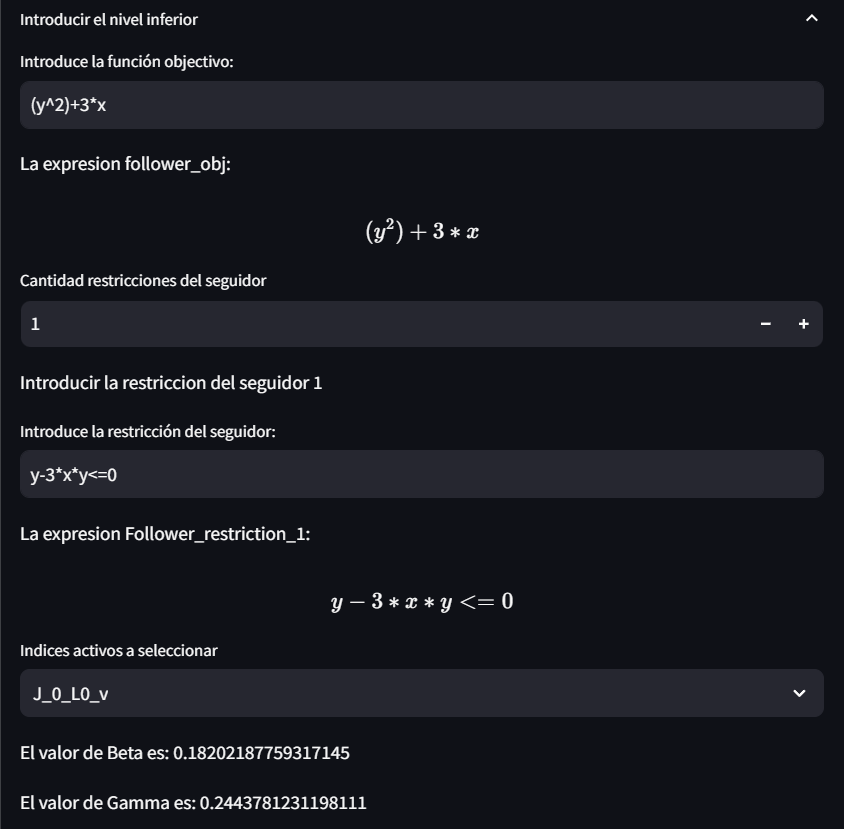
\includegraphics[width=\textwidth]{Graphics/Ejemplo_introducir_follower_rest.png}
    \caption{Ejemplo de generación de problema en punto Fuertemente Estacionario}
    \label{fig:example_strong_stationary_front_generator}
\end{figure}
